\section{Implementacja}

\subsection{Plan implementacji}

Szczegółowe fazy implementacji projektu prezentują się w następujący sposób:

\begin{enumerate}
	\item [1.] Przygotowanie bazy wzorców	
	\begin{itemize}	
		\item Podział nagranych słów na odcinki czasowe o długości 0,05s
		\item Ekstrakcja parametrów słów wzorcowych poprzez FFT oraz bank filtrów
		\item Sprawdzenie powtarzalności wyników dla tego samego słowa, czyli przydatności algorytmu
	\end{itemize}

	\item [2.] Przetestowanie skuteczności programu
	\begin{itemize}	
		\item Nagranie zdań, w których pojawiają się słowa takie, jak w bazie wzorców oraz dodatkowe
		\item Ekstrakcja parametrów dla odcinków zdań i obliczenie korelacji między nimi i słowami wzorcowymi
		\item Wynik: fragmenty, dla których współczynnik korelacji jest większy od zadanego progu zostają uznane za znalezione słowa.
	\end{itemize}
\end{enumerate}

Poszczególne etapy zostały dokładnie opisane w kolejnych punktach dokumentu.


\subsection{Baza wzorców}

Na początku należało wyznaczyć słowa, które mają być wyszukiwane w nagraniach. W tym przypadku zdecydowano się na następujące: ,,książka``, ,,krzesło`` oraz ,,fotel``. \\
Przy gromadzeniu nagrań został uwzględniony fakt, że dla różnych osób rejestrowane parametry dźwięków mogą się różnić. Dlatego swego głosu do celów badawczych udzieliły cztery osoby - po dwie każdej płci. Ostatecznie w bazie znalazły się trzy słowa nagrane przez cztery osoby, po dziewięć razy każde, a więc jeden wyraz został powtórzony 36 razy.


\subsection{Ekstrakcja parametrów}

Po podzieleniu nagranych słów na odcinki odpowiedniej długości poddano je działaniu kilku algorytmów. Pierwszy z nich to szybka transformata Fouriera o 128-miu punktach, a konkretnie część rzeczywista tej transformaty. \\
Dla tak przetworzonych danych można było zastosować bank filtrów. Dla potrzeb projektu wybrano zestaw składający się z 10-ciu filtrów trójkątnych w skali melowej. Dane powstałe w wyniku operacji związanych z FFT przemnożono przez stworzony w ten sposób filtr. Na ilustracji \ref{rys:fftFiltry}. zobrazowano relację, jaka występuje pomiędzy tymi danymi. \\
W wyniku powyższych działań dla każdego słowa otrzymano 

\begin{figure}[H]
	\centering
	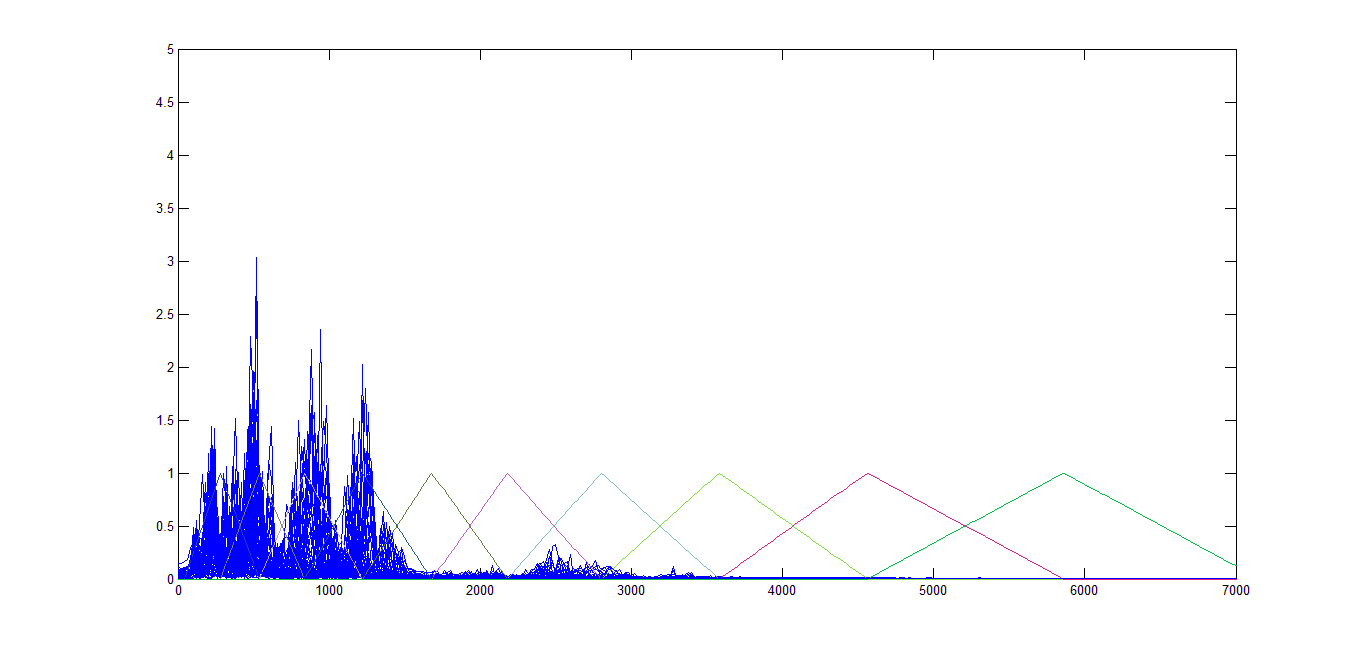
\includegraphics[scale=0.5]{fftFiltersBank}
	\caption{Wynik FFT z nałożonym bankiem filtrów}
	\label{rys:fftFiltry}
\end{figure}